\documentclass{beamer}	
\mode<presentation>
 
\usepackage{pdfpages}
\usepackage{fancyvrb}
\usepackage{chemarr}

\usepackage{amsmath}		%% mathematics typesetting
\usepackage{amssymb}
 
\usepackage{epigraph}   %% nice setting of quotations

\usepackage{tabularx} %% allows to use row colours in tables

\usepackage{ulem}

\usepackage{booktabs}

\usepackage{siunitx} %% tpyeset SI units

\usepackage{CJKutf8} %% typeset Chinese characters

\usepackage{pdfpages}%% include pdfs

\usepackage{graphicx}
\usepackage{animate} %% show animated gifs

\DeclareMathAlphabet{\mathcalligra}{T1}{calligra}{m}{n}


% Color and Theme. Can be changed. However, this one's quite nice.
\usetheme{Madrid}
\definecolor{theme}{rgb}{0.84,0,0.21}
\usecolortheme[named=theme]{structure}

%%  Title information
\title[M11.13.1 Psychophysik]{M11.13.1 Psychophysik: \\ Allgemeine Sinneswahrnehmung}
\author[melanie.stefan@medicalschool-berlin.de]{}
\institute[]{Prof. Melanie Stefan \\ melanie.stefan@medcialschool-berlin.de}
\date{WiSe 2022/23}
 

% Table of contents to pop up at the beginning of each section
\AtBeginSection[]
{
  \begin{frame}<beamer>
    \frametitle{Outline}
    \tableofcontents[currentsection,currentsubsection]
  \end{frame}
}
 
\beamertemplatenavigationsymbolsempty

\begin{document}


{ \usebackgroundtemplate{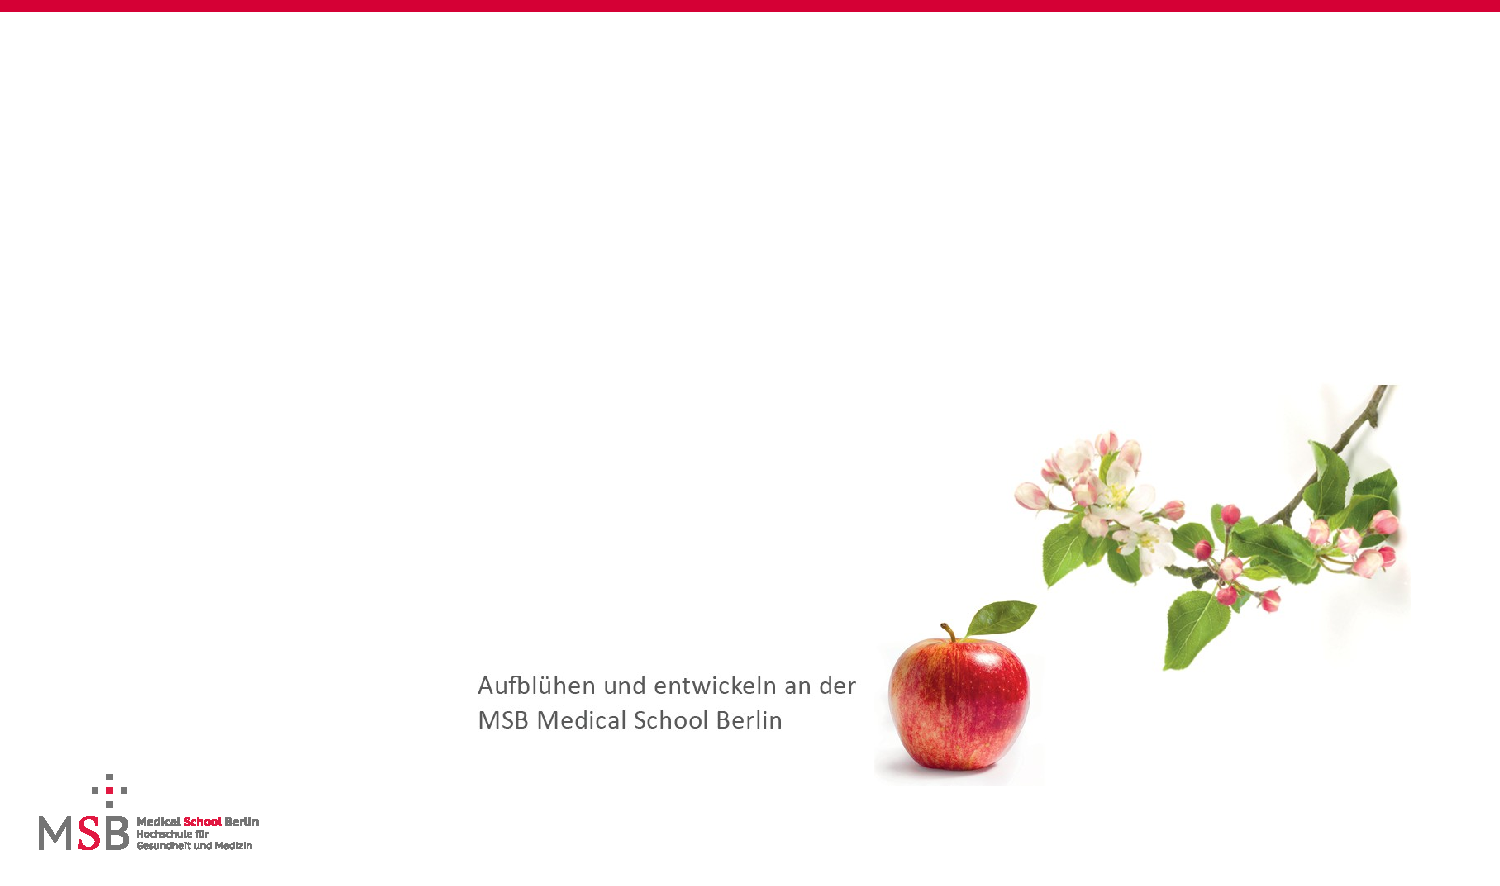
\includegraphics[width=1.2\paperwidth]{MSB_Titelseite.pdf}} 
\begin{frame}

 \maketitle 

$\,$\\[6cm] 


\end{frame} 
}


%% Hook:

{ \usebackgroundtemplate{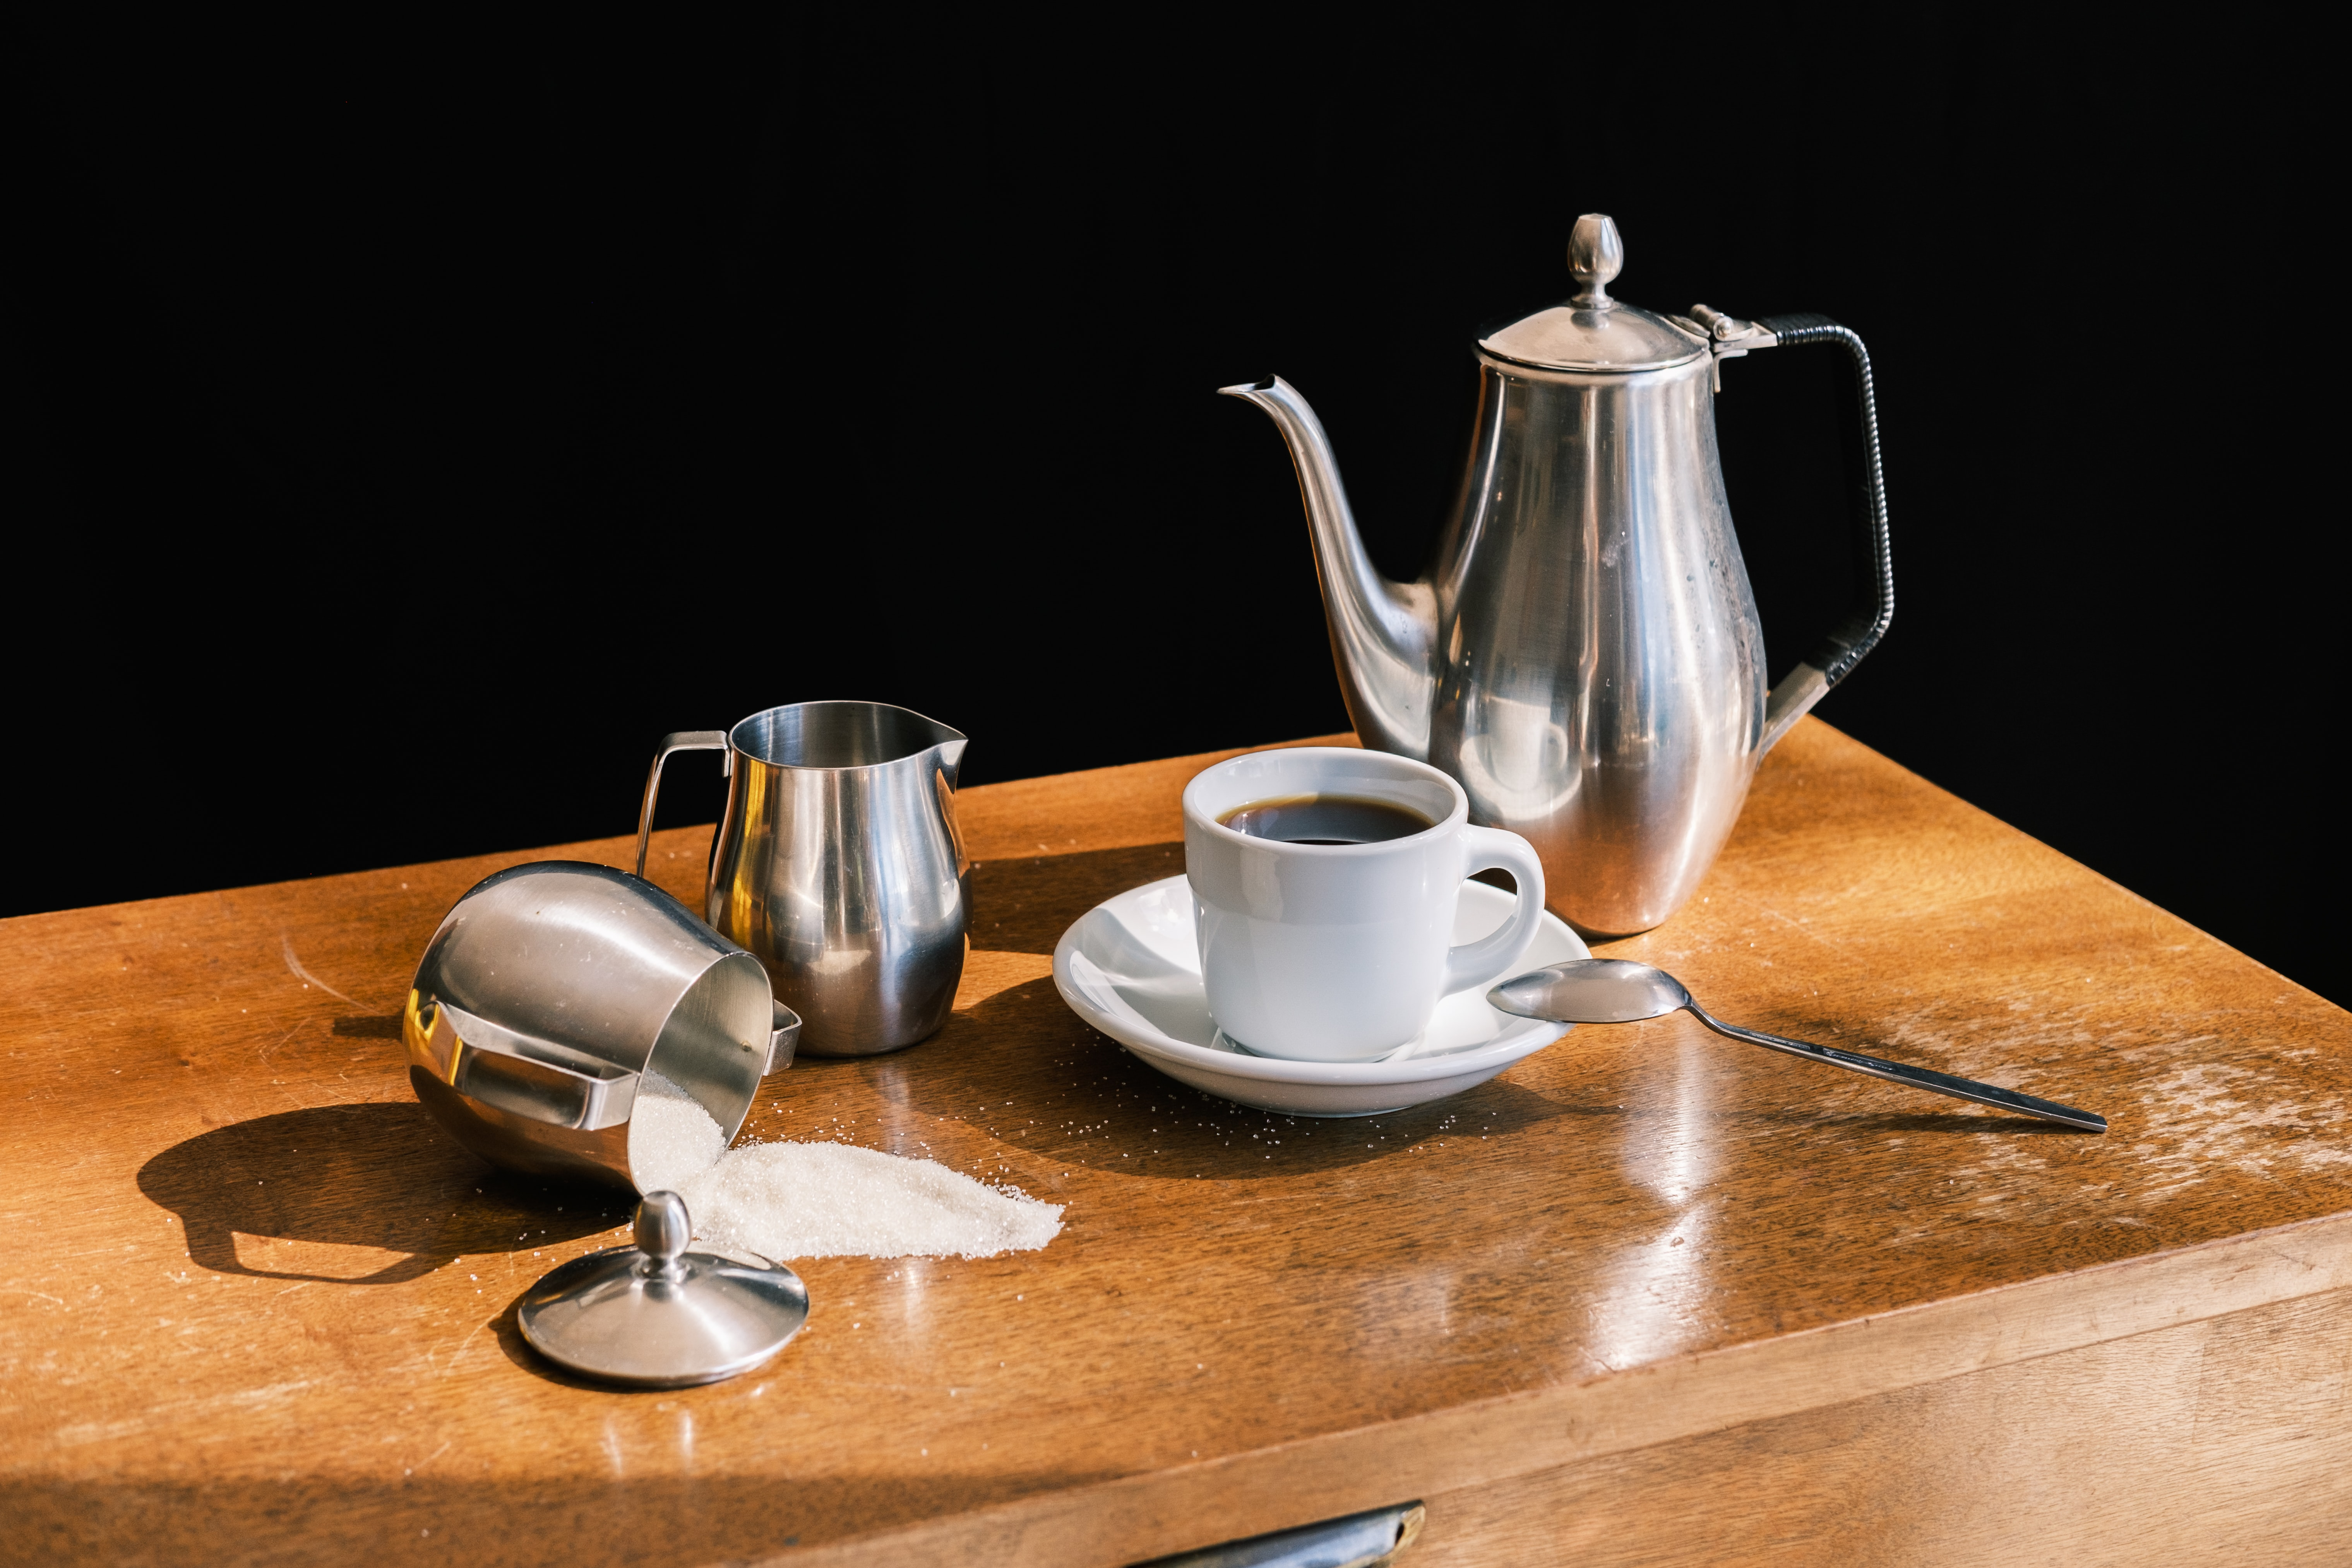
\includegraphics[width=1.2\paperwidth]{still_life.jpg}} 
\begin{frame}
\textcolor{white}{Wir nehmen die Welt durch unsere Sinne wahr \dots}

$\,$\\[3.5cm]

\pause
\textcolor{white}{Aber wie?}

$\,$\\[4cm]

\end{frame}
}

 
% %% %% TLIA
% \begin{frame}{In diesem Semester geht es um Sinnesphysiologie}

% Vorlesungen im 4. Semester:

% \begin{itemize}

% Allgemeine Sinnesphysiologie & Psychophysik und allgemeine Sinnesphysiologie \\
% Somatosensorik & Somatosensorik 1: Tastsinn \\
%     & Somatosensorik 2: Propriozeption und Thermorezeption \\
%     & Somatosensorik 3: Nozizeption und Schmerz \\
% Visuelles System & Visuelles System 1: Dioptrischer Apparat \\
%     & Visuelles System 2: Retinale Signalverarbeitung, zentrale Sehbahn \\
%     Gehör und Gleichgewicht & Auditorisches System: Hören und periphere Hörbahnen \\
%     & Vestibuläres System \\
    
%     Chemische Sinne & Chemosensorik: Geschmack und Geruch \\
% \end{itemize}

% \pause

% (Der Rest sind Repetitorien)

% \end{frame}


%%  % Learning Objectives
 
% \begin{frame}

%  \frametitle{Nach dieser Vorlesung sollten Sie folgendes können}



% \begin{block}{Grundlagen:}

% \begin{itemize}
    
% \item 
% Aufbau und Funktionsweise von Skelettmuskeln erklären
% \item
% die sensorischen Funktionen von Muskelspindeln und Golgi-Sehnen-Organ erklären 
% \item
% den Aufbau des  Vestibularsytems erklären
% \item
% Nuclei des Kleinhirns benennen und ihre Funktion erklären
% \item
% Aufbau und Vernetzung der Schichten des Kleinhirnkortex erläutern
% \item
% Funktion und Organisation des Rückenmarks erklären
% \item
% Reflexe der Skelettmuskulatur erklären 
% \item
% Beispiele für supraspinale Reflexe geben
% \end{itemize}


% \end{block}


% \end{frame}


 
% \begin{frame}

%  \frametitle{Nach dieser Vorlesung sollten Sie folgendes können}

% \begin{block}{Klinik:}

% \begin{itemize}
    
% \item 
% Pathologien bei Störung des Kleinhirns benennen und erklären
% \item
% Reflexe hervorrufen und zur Diagnose einsetzen (Praktikum!)
% \end{itemize}


% \end{block}



% \end{frame}









%% %% %% Main Body
 


%% %% %% %% Review






%% %% %% %% Feedbackhinweisblock

\begin{frame}
\frametitle{Danke für Ihr Feedback!}

\begin{columns}[c]

\begin{column}{6cm}
\begin{center}
 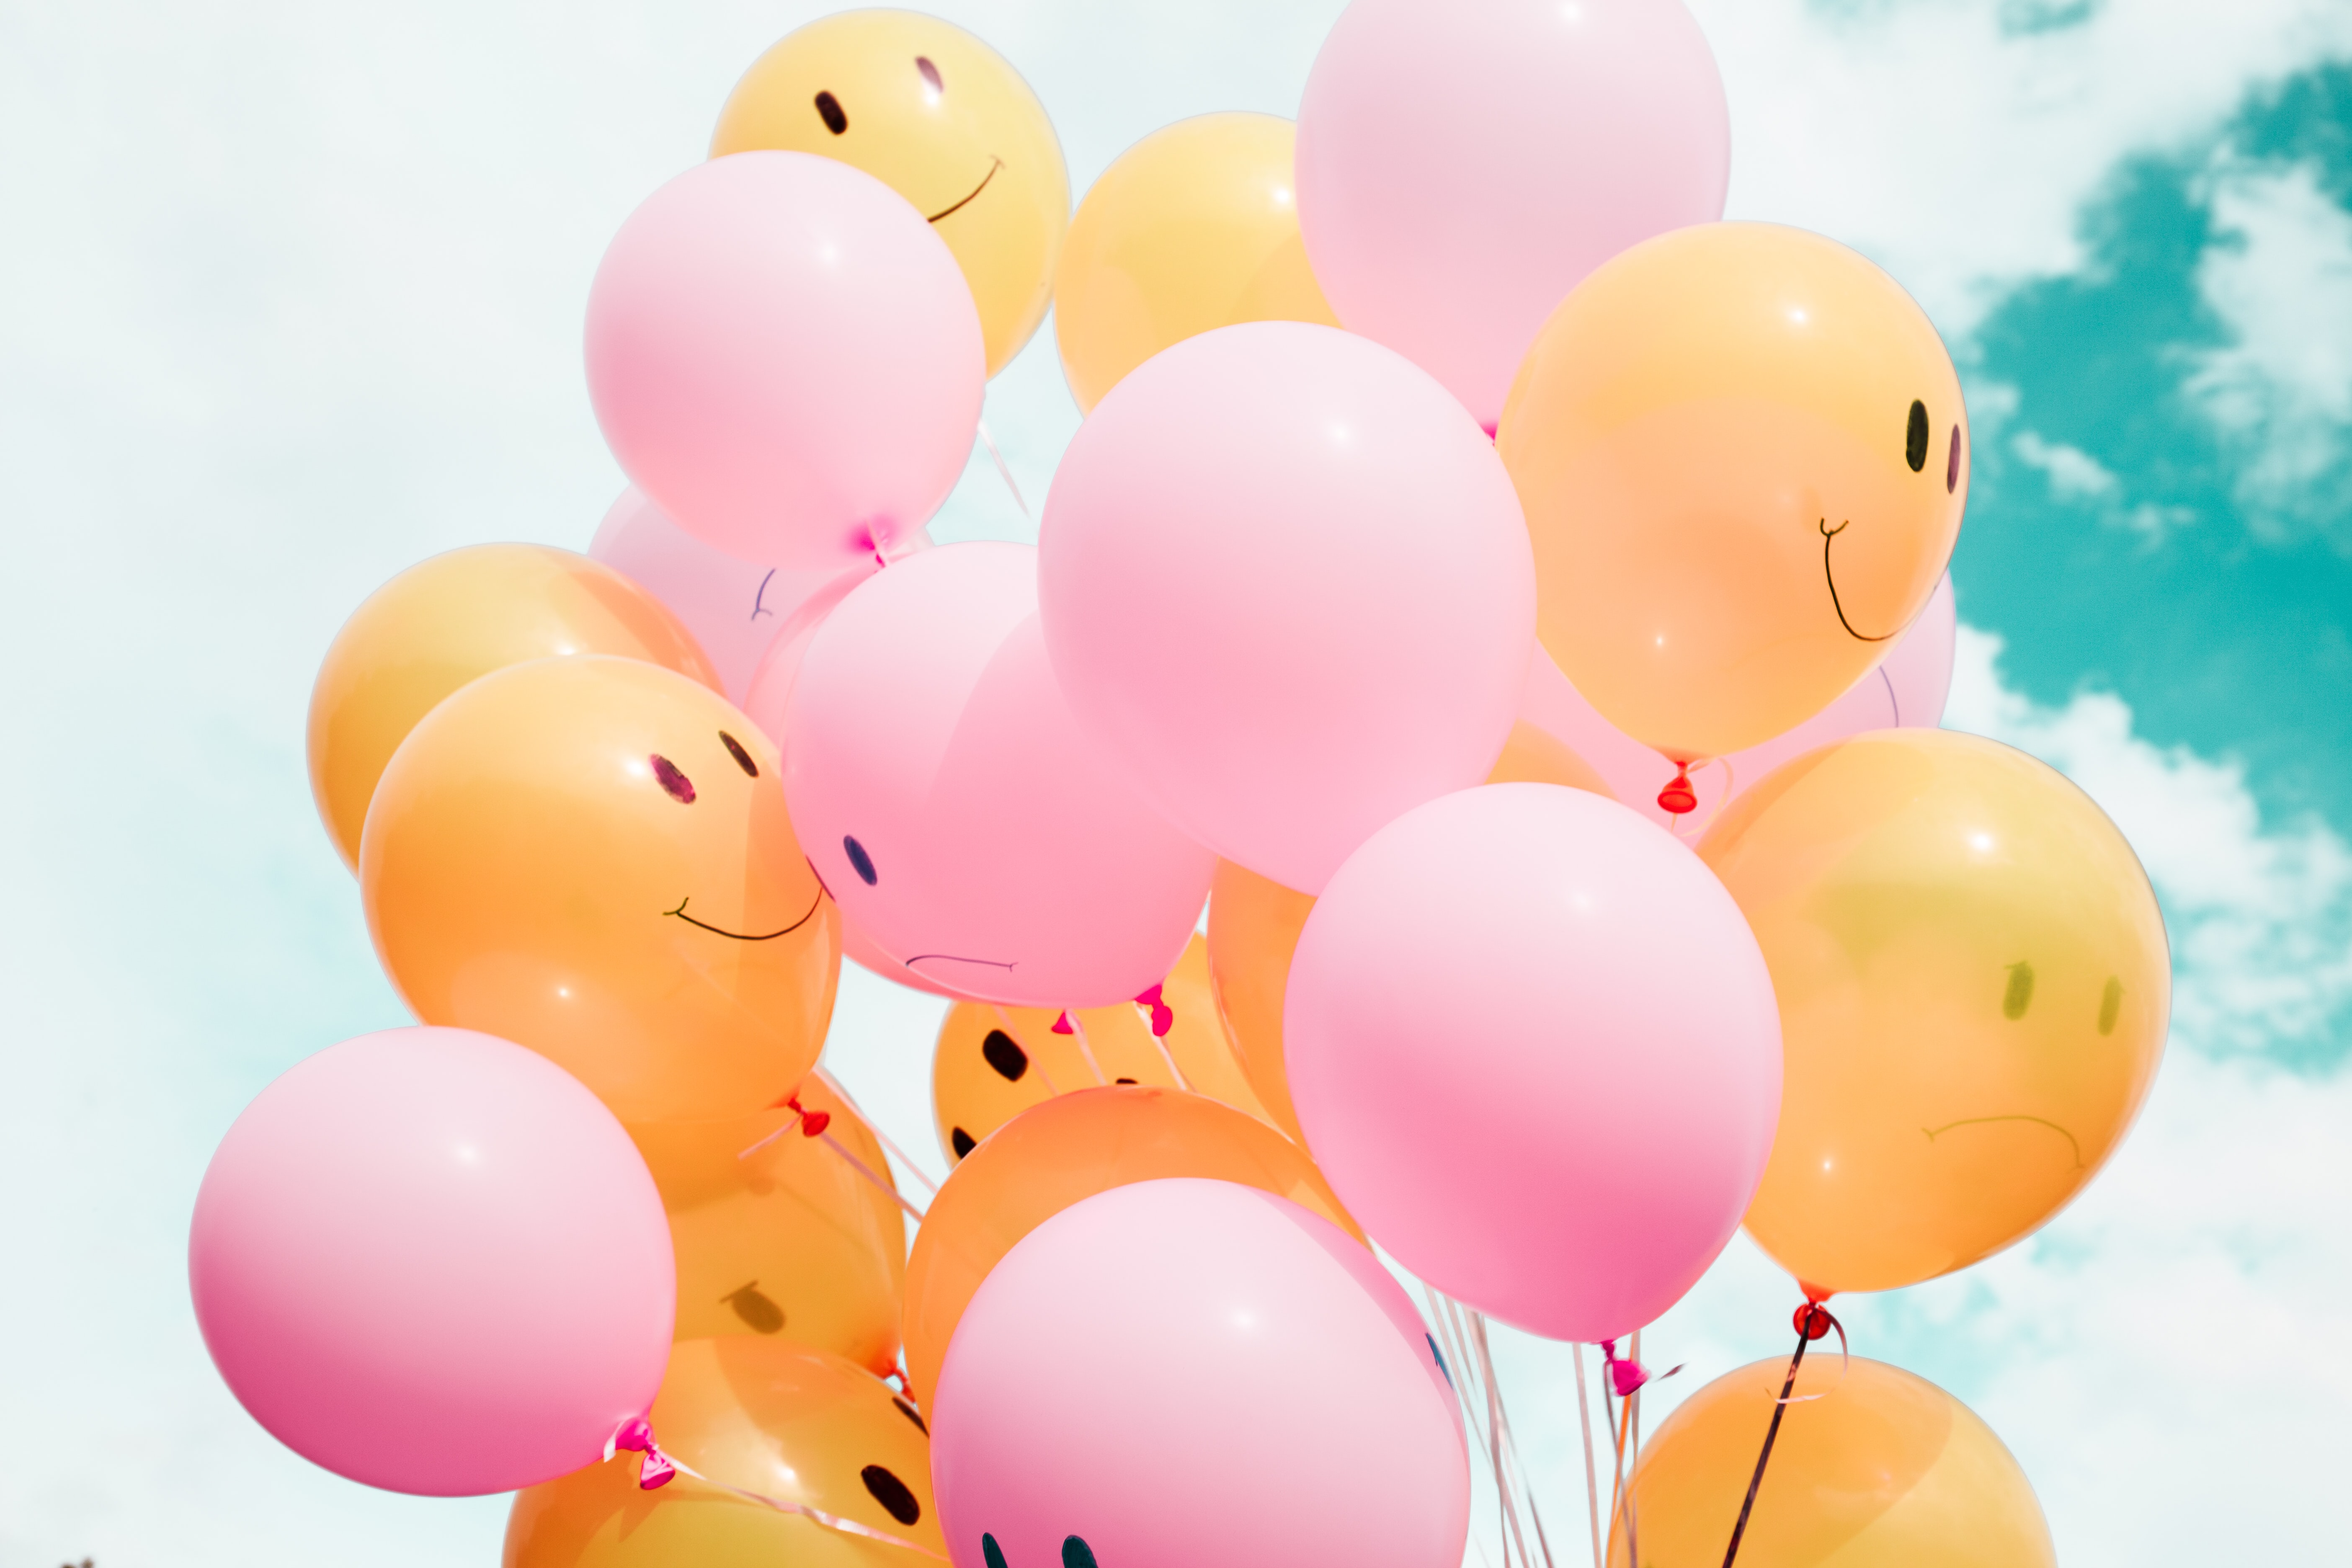
\includegraphics[width=\textwidth]{smilie_balloons.jpg}
\end{center}

\end{column}

\begin{column}{4cm}


\begin{center}

\includegraphics[width=\textwidth]{feedback_QR.png}
\end{center}
\end{column}


\end{columns}
\end{frame}




%% %% %% Bildnachweis
\begin{frame}
\frametitle{Bildnachweis}
\begin{tiny}

% Teile dieser Vorlesung wurden übernommen von einer Vorlesung von Prof. Maike Glitsch, Medical School Hamburg, der wir an dieser Stelle herzlich danken. Wo nicht anders gekennzeichnet, stammen Abbildungen aus dieser Vorlesung.  


 
\begin{itemize}

\item
Luftballons mit frohen und traurigen Smileys. Photo by \href{https://unsplash.com/@artbyhybrid?utm_source=unsplash&utm_medium=referral&utm_content=creditCopyText}{Hybrid} on \href{https://unsplash.com/s/photos/feedback?utm_source=unsplash&utm_medium=referral&utm_content=creditCopyText}{Unsplash}


\item
Stillleben mit Kaffee. Photo by \href{https://unsplash.com/@garrethpb?utm_source=unsplash&utm_medium=referral&utm_content=creditCopyText}{Garreth Paul} on \href{https://unsplash.com/s/photos/still-life?utm_source=unsplash&utm_medium=referral&utm_content=creditCopyText}{Unsplash}
  
\end{itemize}
\end{tiny}
\end{frame}






\end{document}

%%% Frequently used snippets

%% \begin{columns}[c]

%% \begin{column}{5cm}
%% \end{column}

%% \begin{column}{5cm}
%% \end{column}


%% \end{columns}




